\documentclass[11pt,a4paper]{article}
\usepackage[margin=23mm]{geometry}
\usepackage[T1]{fontenc}
\usepackage{lmodern}
\usepackage{hyperref}
\usepackage{tikz}
\usetikzlibrary{positioning,arrows.meta}
\title{Core: refresh the shared contract consumer}
\date{Created-at: 2026-09-05 19:53 +02:00}
\begin{document}
\maketitle
\paragraph{Scope and authorization.}
The user explicitly requested applying the updated hymeko/hymeko repository
here. Adopt the fetched default-branch provider revision
\texttt{5517e6b3b63df3e9632b1fb810a41470b51a2f73} into the existing
Core audit checkout at \texttt{8a0c49d}. Core is ahead 24, behind 0 of its
fresh origin/main; both owner repositories were successfully fetched at 19:53.
ETA: 10--20 minutes for entry-point wiring, existing hook/pin refresh, consumer
checks and the report. No product source, Rust dependency or fixture changes.
\paragraph{Discovery and ownership.}
Core already owns CLAUDE.md, SYMBOLS.md, tools/hooks, a duplication baseline,
and a workflow template. Reuse them. AGENTS.md and .claude/settings.json are
absent; the provider rollout requires a repository-local entry point. The
provider owns shared rules and tools: reference those rather than vendor them.
Move only this task's clean provider checkout from sibling provider to sibling
hymeko after path containment and cleanliness checks; no additional checkout.
\paragraph{Files.}
Add AGENTS.md and .claude/settings.json; update CLAUDE.md,
docs/agent-contract/README.md, docs/agent-contract/repo/toolchain.md,
tools/hooks/pre-commit, tools/hooks/commit-msg,
.github/workflows/duplication-gate.yml and SYMBOLS.md.
Preserve the existing hook installer and provider-only self-check guard.
Add this plan quartet, reports/2026-09-05-contract-provider-refresh.md,
reports/contract-provider-refresh/ verification evidence, and .gitattributes
entries preserving these bytes. The already-staged admission evidence remains
a separate thematic commit; its generated-index refresh can precede adoption.
\paragraph{Contracts and risk.}
CORE.YAML protected items touched: empty. The tooling remains version 0.1.0;
the user explicitly directed its revision refresh. Existing Core ownership,
resource and approval rules remain. Retain historical copied modules for old
citations but mark the external provider as current authority. Never impose the
provider-only aggregate suite on Core. A global installed tool can drift from
the consumer pin; verify actual installation provenance and report that limit.
External Claude imports need project trust; file checks cannot prove a separate
Claude session has accepted them. No unsupported claim of active remote CI.
\paragraph{Verification and budgets.}
Compile this plan before editing entry points. Compare old installed hooks before
replacement, install the exact provider revision, and require current status.
Read changed index ownership grouping; retain unchanged duplication baseline.
Run symbols and duplication explicitly. Exercise real staged-path preflight
using temporary commit-message files: missing DISCOVERY blocks and a justified
DISCOVERY releases. Verify settings JSON, import targets and pin consistency.
Use existing provider persona tests/entry point for the adapted Stop command.
No new permanent test harness. Bound diagnostic checks to under five minutes
and 2 GiB working set; measure gate wall time against the existing two-second
hook target. No performance or formal Core remeasurement: product bytes match
the already verified 8a0c49d image.
\paragraph{Rollback and acceptance.}
Update at 2026-09-05 20:02 +02:00: provider main advanced during migration to
\texttt{d02aa614bc06a348dbcbe3936dcd3b9285b8bdeb}. Fetch succeeded and the clean
sibling was fast-forwarded. The new global task-continuity and completion rules
were read in full. The portable gate implementations are unchanged; final pins,
installation and consumer checks will use this newer immutable revision. Preserve
the 5517e6b checks as intermediate evidence rather than relabel them.

Revert only the scoped consumer-adoption commit and reinstall its prior hooks;
do not overwrite unrelated global configuration or user changes. Record source
revisions, file deltas, gate results and actual activation limits. This work does
not publish, merge or tag repositories; dependency integration follows the
user's preceding direction after its protected scopes are made reviewable.
\begin{center}
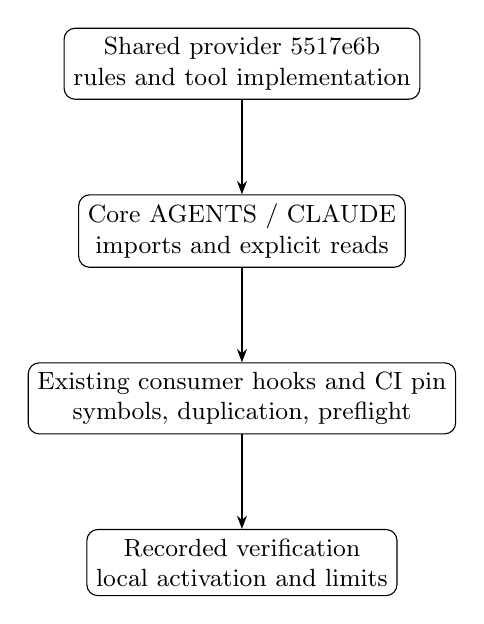
\begin{tikzpicture}[node distance=12mm, every node/.style={draw,rounded corners,align=center,font=\small}, >={Stealth}]
\node (p) {Shared provider 5517e6b\\rules and tool implementation};
\node (e) [below=of p] {Core AGENTS / CLAUDE\\imports and explicit reads};
\node (g) [below=of e] {Existing consumer hooks and CI pin\\symbols, duplication, preflight};
\node (r) [below=of g] {Recorded verification\\local activation and limits};
\draw[->] (p)--(e); \draw[->] (e)--(g); \draw[->] (g)--(r);
\end{tikzpicture}
\end{center}

\end{document}
